\documentclass[11pt]{article}
\usepackage[margin=1in]{geometry}
\usepackage{amsmath,amssymb,amsthm}
\usepackage{enumitem}
\usepackage{graphicx}
\usepackage[hidelinks]{hyperref}

\title{Joint J-Strict Continuity of the Multiplier Jordan Product}
\author{Candidate full solution for the FA/Banach discovery run}
\date{23 July 2026}

\newtheorem{theorem}{Theorem}
\newtheorem{lemma}[theorem]{Lemma}
\newtheorem{corollary}[theorem]{Corollary}
\newtheorem*{remark}{Remark}
\newcommand{\A}{\mathfrak A}
\newcommand{\M}{M(\mathfrak A)}
\newcommand{\one}{\mathbf 1}
\newcommand{\sa}{\mathrm{sa}}

\begin{document}
\maketitle

\section*{Source questions and answer}

The source is Fernandez-Polo, Garces, Li, and Peralta,
\emph{On the strict topology of the multipliers of a JB$^*$-algebra},
arXiv:2210.13353 \cite{FGLP}. On page 25 it asks:
\begin{enumerate}[label=(Q\arabic*),leftmargin=*]
\item Is the Jordan product of \(M(\A)\) separately J-strict continuous
      (on bounded sets)?
\item Is the Jordan product of \(M(\A)\) jointly J-strict continuous on
      bounded sets?
\end{enumerate}
Both answers are affirmative. The source page is included as
\texttt{source\_paper.pdf}; the exact statement is reproduced below.

\begin{center}
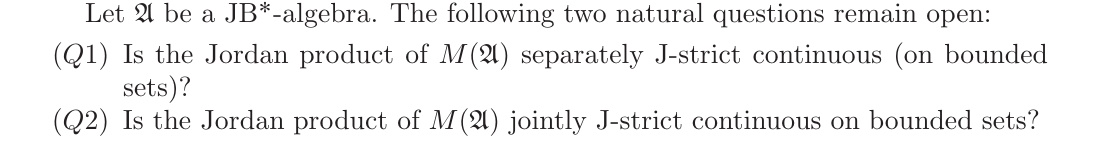
\includegraphics[width=\textwidth]{figures/open_questions_crop.png}
\end{center}

A bounded search on 23 July 2026 used the arXiv id, exact title, exact
question phrases, \emph{Jordan product J-strict topology multipliers}, and
the published DOI \nolinkurl{10.1007/s13398-023-01476-w}, including
citation-oriented variants. It found the source and bibliographic mirrors but
no later work claiming either answer. This is bounded negative evidence, not
a comprehensive novelty guarantee.

\section*{Notation and standard facts}

Let \(\A\) be a JB$^*$-algebra and let \(\M\) be its unital multiplier
JB$^*$-algebra. Its J-strict topology is generated by
\[
 \rho_a(z)=\lVert z\circ a\rVert,\qquad a\in\A,\ z\in\M.
\]
The source proves that J-strict bounded sets in \(\M\) are exactly the
norm-bounded sets \cite{FGLP}. It also recalls that \(\A\) has a positive
contractive approximate unit \((e_\gamma)\) such that
\begin{equation}\label{eq:approx-tail}
 \lVert U_{\one-e_\gamma}(a)\rVert\longrightarrow0
 \qquad(a\in\A).
\end{equation}

For elements of a Jordan algebra, write
\[
 U_x(t)=2(x\circ t)\circ x-x^2\circ t
\]
and introduce the symmetric bilinearization
\[
 U_{x,y}(t)
 =(x\circ t)\circ y+(y\circ t)\circ x-(x\circ y)\circ t.
\]
Thus \(U_{x+y}=U_x+U_y+2U_{x,y}\), and norm
submultiplicativity gives
\begin{equation}\label{eq:bilinear-bound}
 \lVert U_{x,y}(t)\rVert
 \leq3\lVert x\rVert\lVert y\rVert\lVert t\rVert.
\end{equation}
We use the fundamental identity
\begin{equation}\label{eq:fundamental}
 U_{U_x(y)}=U_xU_yU_x
\end{equation}
and the standard JB inequality
\begin{equation}\label{eq:JB-inequality}
 \lVert a\circ b\rVert^2
 \leq \lVert a\rVert\,\lVert U_b(a)\rVert
 \quad(a\geq0,\ b=b^*).
\end{equation}
These are precisely the two standard facts recalled in the source
\cite{FGLP,HOS}.

\section*{Proof intuition}

Fix a positive contractive approximate-unit element \(e\), and put
\(c=\one-e\). Split a multiplier \(z\) into
\[
 z=L_ez+R_ez,\qquad R_ez=U_cz.
\]
The local part \(L_ez\) belongs to \(\A\), and if \(z\) tends J-strictly to
zero then \(L_ez\) tends to zero in norm for this fixed \(e\). The remaining
tail is not norm-small, but products of two tails remain tails:
\[
 U_cx\circ U_cy=U_c\bigl(U_{x,y}(c^2)\bigr).
\]
The JB inequality and the fundamental identity estimate this last expression
against \(\lVert U_c(a)\rVert\) for each positive test element \(a\in\A\).
Equation \eqref{eq:approx-tail} makes that quantity uniformly small on
norm-bounded \(x,y\). This is the Jordan substitute for moving an element of
an associative ideal through a product.

\section*{Localization lemmas}

\begin{lemma}[local-tail decomposition]\label{lem:decomp}
Let \(e\in\A\) be a positive contraction and put \(c=\one-e\). For every
\(z\in\M\),
\[
 R_ez:=U_cz,\qquad
 L_ez:=z-U_cz
 =2e\circ z-2(e\circ z)\circ e+e^2\circ z.
\]
In particular \(L_ez\in\A\), and
\begin{equation}\label{eq:local-bound}
 \lVert L_ez\rVert
 \leq4\rho_e(z)+\rho_{e^2}(z).
\end{equation}
\end{lemma}

\begin{proof}
Since \(c=\one-e\), direct expansion of the quadratic representation gives
\[
 U_cz=z-2e\circ z+2(e\circ z)\circ e-e^2\circ z.
\]
The multiplier property puts \(e\circ z\) and \(e^2\circ z\) in \(\A\);
hence \(L_ez\in\A\). The displayed norm estimate follows from
\(\lVert e\rVert\leq1\) and norm submultiplicativity.
\end{proof}

\begin{lemma}[uniform quadratic-tail estimate]\label{lem:tail}
Let \(c=c^*\) be a contraction in \(\M\), \(w=w^*\in\M\), and
\(a\in\A_+\). Then
\begin{equation}\label{eq:tail-estimate}
 \lVert U_cw\circ a\rVert^2
 \leq\lVert a\rVert\,\lVert w\rVert^2\lVert U_c(a)\rVert.
\end{equation}
\end{lemma}

\begin{proof}
Apply \eqref{eq:JB-inequality} with \(b=U_cw\), then use
\eqref{eq:fundamental}:
\[
\begin{aligned}
\lVert U_cw\circ a\rVert^2
 &\leq\lVert a\rVert\,\lVert U_{U_cw}(a)\rVert\\
 &=\lVert a\rVert\,\lVert U_cU_wU_c(a)\rVert\\
 &\leq\lVert a\rVert\,\lVert c\rVert^2
       \lVert w\rVert^2\lVert U_c(a)\rVert.
\end{aligned}
\]
Here \(\lVert U_v\rVert\leq\lVert v\rVert^2\), and
\(\lVert c\rVert\leq1\).
\end{proof}

\begin{lemma}[tail-product identity]\label{lem:tail-product}
For \(c,x,y\) in a unital Jordan algebra,
\begin{equation}\label{eq:tail-product}
 U_cx\circ U_cy=U_c\bigl(U_{x,y}(c^2)\bigr).
\end{equation}
\end{lemma}

\begin{proof}
Apply the fundamental identity to the unit:
\[
 (U_cz)^2=U_{U_cz}(\one)=U_cU_zU_c(\one)=U_c\bigl(U_z(c^2)\bigr).
\]
Substitute \(z=x+y\), subtract the corresponding formulas for \(x\) and
\(y\), and use
\[
 (r+s)^2-r^2-s^2=2r\circ s,\qquad
 U_{x+y}-U_x-U_y=2U_{x,y}.
\]
Dividing by \(2\) gives \eqref{eq:tail-product}. Thus the identity uses only
the fundamental Jordan identity and is valid also in exceptional Jordan
algebras.
\end{proof}

Combining Lemmas \ref{lem:tail} and \ref{lem:tail-product} with
\eqref{eq:bilinear-bound} gives the estimate that drives the proof:
if \(x,y\in\M_\sa\), \(\lVert x\rVert,\lVert y\rVert\leq C\), and
\(c\) is a self-adjoint contraction, then for \(a\in\A_+\),
\begin{equation}\label{eq:tail-tail}
\begin{aligned}
 \rho_a(U_cx\circ U_cy)^2
 &=\left\lVert
 a\circ U_c\bigl(U_{x,y}(c^2)\bigr)\right\rVert^2\\
 &\leq9C^4\lVert a\rVert\,\lVert U_c(a)\rVert.
\end{aligned}
\end{equation}

\section*{Main theorem}

\begin{theorem}\label{thm:main}
Let \(\A\) be a JB$^*$-algebra.
\begin{enumerate}[label=(\roman*),leftmargin=*]
\item The Jordan product on \(\M\) is separately J-strict continuous.
\item If \(x_\lambda\to x\) and \(y_\mu\to y\) J-strictly and both nets are
      norm bounded, then
      \[
       x_\lambda\circ y_\mu\longrightarrow x\circ y
      \]
      J-strictly on the product directed set.
\end{enumerate}
Consequently Questions Q1 and Q2 both have affirmative answers.
\end{theorem}

\begin{proof}
We first work in the self-adjoint part and test against \(a\in\A_+\).

\smallskip
\noindent\emph{Joint continuity at \((0,0)\).}
Suppose \(x_\lambda\to0\) and \(y_\mu\to0\) J-strictly, with
\(\lVert x_\lambda\rVert,\lVert y_\mu\rVert\leq C\). Let
\((e_\gamma)\) be a positive contractive approximate unit and set
\(c_\gamma=\one-e_\gamma\). For a fixed \(\gamma\), Lemma
\ref{lem:decomp} gives
\[
 \lVert L_{e_\gamma}x_\lambda\rVert\longrightarrow0,\qquad
 \lVert L_{e_\gamma}y_\mu\rVert\longrightarrow0.
\]
Using \(x_\lambda=L_ex_\lambda+R_ex_\lambda\), and suppressing the fixed
subscript \(\gamma\), write
\[
 x_\lambda\circ y_\mu
 =(L_ex_\lambda)\circ y_\mu
 +(R_ex_\lambda)\circ(L_ey_\mu)
 +(R_ex_\lambda)\circ(R_ey_\mu).
\]
The first two terms tend to zero in norm on the product directed set:
\[
\begin{aligned}
 \lVert(L_ex_\lambda)\circ y_\mu\rVert
 &\leq C\lVert L_ex_\lambda\rVert,\\
 \lVert(R_ex_\lambda)\circ(L_ey_\mu)\rVert
 &\leq C\lVert L_ey_\mu\rVert.
\end{aligned}
\]
For the last term, \eqref{eq:tail-tail} says
\[
 \rho_a\bigl((R_ex_\lambda)\circ(R_ey_\mu)\bigr)^2
 \leq9C^4\lVert a\rVert\,\lVert U_{\one-e}(a)\rVert.
\]
Given \(\varepsilon>0\), first choose \(\gamma\) so that the right-hand side
is smaller than \(\varepsilon^2/9\), using
\eqref{eq:approx-tail}. With this \(e=e_\gamma\) fixed, choose
\(\lambda,\mu\) late enough that the first two terms contribute less than
\(2\varepsilon/3\) after applying \(\rho_a\). Hence
\(\rho_a(x_\lambda\circ y_\mu)\to0\).

\smallskip
\noindent\emph{Separate continuity at zero.}
Fix \(x=x^*\in\M\), and let \(z_\lambda=z_\lambda^*\to0\) J-strictly with
\(\lVert z_\lambda\rVert\leq C\). Decompose with the same \(e,c\):
\[
 x\circ z_\lambda
 =(L_ex)\circ z_\lambda
 +(R_ex)\circ(L_ez_\lambda)
 +(R_ex)\circ(R_ez_\lambda).
\]
Because \(L_ex\in\A\),
\[
 \lVert(L_ex)\circ z_\lambda\rVert=\rho_{L_ex}(z_\lambda)\longrightarrow0.
\]
The second term tends to zero in norm by Lemma \ref{lem:decomp}. For the
third, the proof of \eqref{eq:tail-tail} gives
\[
 \rho_a\bigl((R_ex)\circ(R_ez_\lambda)\bigr)^2
 \leq9\lVert x\rVert^2C^2\lVert a\rVert
       \lVert U_{\one-e}(a)\rVert.
\]
Choose \(e\) late in the approximate unit and then \(\lambda\) late. This
proves \(x\circ z_\lambda\to0\) J-strictly.

\smallskip
\noindent\emph{All test elements and complex elements.}
Every self-adjoint \(a\in\A\) is a difference of two positive elements, and
every element of \(\A\) is a complex linear combination of self-adjoint
elements. Thus positive test elements determine J-strict convergence.
Moreover
\[
 \rho_a(z^*)=\rho_{a^*}(z).
\]
Consequently the real and imaginary parts of a bounded J-strict-null net are
bounded J-strict-null self-adjoint nets. Expanding the Jordan product
complex-bilinearly reduces both assertions just proved to the self-adjoint
case.

\smallskip
\noindent\emph{Arbitrary limits.}
For bounded J-strictly convergent nets, the difference nets are bounded, and
\[
\begin{aligned}
x_\lambda\circ y_\mu-x\circ y
={}&(x_\lambda-x)\circ(y_\mu-y)\\
&+x\circ(y_\mu-y)+(x_\lambda-x)\circ y.
\end{aligned}
\]
The first term tends to zero by joint continuity at \((0,0)\), and the last
two by separate continuity. This proves (ii).

Finally, every J-strictly convergent net is J-strict bounded and hence norm
bounded by the bounded-set theorem in \cite{FGLP}. The separate-continuity
argument therefore applies to every convergent net, proving (i).
\end{proof}

\section*{Verification notes}

\begin{itemize}[leftmargin=*]
\item The proof is internal to Jordan algebra theory. It does not embed
      \(\A\) into an associative algebra, so exceptional JB$^*$-algebras are
      covered.
\item As an independent guard against a special-only identity, the
      fundamental identity and \eqref{eq:tail-product} were evaluated in 40
      exact random trials in the exceptional 27-dimensional real Albert
      algebra. The script is included as
      \texttt{code/check\_albert\_identities.py}. Computation is only a sanity
      check; Lemma \ref{lem:tail-product} is the proof.
\item The source crop is reproducible with
      \texttt{code/make\_open\_questions\_crop.py}.
\item The bounded novelty search cannot exclude an unindexed or differently
      phrased answer. Novelty confidence is therefore moderate.
\end{itemize}

\begin{thebibliography}{9}
\bibitem{FGLP}
F. J. Fernandez-Polo, J. J. Garces, L. Li, and A. M. Peralta,
\emph{On the strict topology of the multipliers of a JB$^*$-algebra},
Rev. R. Acad. Cienc. Exactas Fis. Nat. Ser. A Mat. RACSAM
\textbf{117} (2023), Paper No. 146; arXiv:2210.13353.

\bibitem{HOS}
H. Hanche-Olsen and E. St{\o}rmer,
\emph{Jordan Operator Algebras}, Pitman, London, 1984.
\end{thebibliography}

\end{document}
